%
% Extended abstract -- Model collapse and the induction-head circuit
% Based on the CCN two-page summary template (ccn_style.tex).
%
% DRAFT. Every number below is produced by experiments/analyze_results.py
% from results/ (see results/analysis_summary.json). Compile on Overleaf (no
% LaTeX engine was available where this was drafted) and check the page
% count: the body must fit the two-page limit. If it overflows, cut in this
% order: (1) the Background sentence on circuit-discovery tools, (2) the
% "Diagnostics" detail in Methods, (3) the Discussion limitations (they are
% repeated in full in the Supplementary Material), (4) Fig. 1(b).
%
\documentclass[10pt,letterpaper]{article}

\usepackage{ccn}
\usepackage{pslatex}
\usepackage{apacite}
\usepackage{graphicx}
\usepackage{caption}
\usepackage{natbib}
\usepackage{float}

\usepackage{hyperref}
\usepackage{url}
\usepackage{booktabs}
\usepackage{amsfonts}
\usepackage{nicefrac}
\usepackage{microtype}
\usepackage{xcolor}
\usepackage{amsmath}
\usepackage{amssymb}
\usepackage{mathtools}
\usepackage{amsthm}
\usepackage[labelfont=bf, margin=0.8cm, font=sf]{caption}

\title{Model Collapse Abruptly Removes the Induction Circuit: A Mechanistic Study on a Synthetic In-Context Learning Task}

% TODO(author): replace with the real author name(s), 1--3 people.
\author{{\large \bf [Author 1]} \\ University of the Witwatersrand, 1 Jan Smuts Ave,\\ Braamfontein, Johannesburg, 2000, South Africa}
% \AND {\large \bf [Author 2]} \\ University of the Witwatersrand, ...

\begin{document}

\maketitle
% NOTE(author): the next four lines are verbatim from the course template.
% They typeset blank pages before the Abstract; check on Overleaf that this
% matches what the course expects before submitting.
\phantom{.}
\newpage
\phantom{.}
\newpage

\section{Abstract}
{
\bf
\looseness=-1
Training on model-generated data risks \emph{model collapse}, while much
in-context learning (ICL) relies on \emph{induction heads}. Does collapse
degrade this circuit? We train small transformers on a few-shot symbol task
that only in-context induction can solve, and run 10-generation
fit$\to$sample$\to$refit pipelines in a base variant (the model relabels
real contexts) and an extended variant (it generates whole sequences), with
3 seeds and a data-mixing ablation. Collapse is abrupt, not gradual: with
fully synthetic data the extended model's accuracy falls from 99.5\% to
$\approx$20\% within 1--4 generations in every seed and never recovers, and
induction scores drop to the random-attention baseline. Failed models fit
their training pool (train accuracy 0.96) but do not generalise
(validation $\approx$0.27): memorisation replaces induction. Marginal symbol
statistics barely move and miss the failure. With 25\% synthetic data 26 of
27 trained models were healthy, but the base variant is not immune.
}
\begin{quote}
\small
\textbf{Keywords:} induction heads; model collapse; mechanistic interpretability
\end{quote}

\section{Introduction} \label{Intro}
\looseness=-1
Models are increasingly trained on text produced by earlier models.
\citet{shumailov2023curse,shumailov2024ai} show that recursively fitting
generation $n$ to samples from generation $n{-}1$ erodes the tails of the
learned distribution until outputs are homogeneous. This is measured through
output statistics; what happens \emph{inside} the model is little studied.
We study the \emph{induction head}: a previous-token head feeding a later
head that attends to what followed an earlier occurrence of the current
token and copies it. \citet{olsson2022incontext} argue this circuit
underlies much ICL, and \citet{singh2024needs} study how it forms, abruptly,
on a synthetic few-shot task. We adopt that task because per-sequence
relabelling forbids memorising an exemplar$\to$label table: accuracy that
survives must come from in-context induction. Circuit-discovery work
motivates our diagnostics (ACDC, \citealp{conmy2023towards}; training-data
attribution, \citealp{chen2026mechanistic}), though we implement only
simplified versions. \textbf{Does recursive training on synthetic data
degrade the induction circuit, is it replaced by memorisation, and does
distributional drift predict it?}

\section{Methods}
\looseness=-1
\textbf{Task.} Each sequence shows 4 distinct exemplars ($K{=}64$ symbol
IDs), 3 times each in random order, each paired with a label ($L{=}8$) drawn
afresh for that sequence; a query exemplar's label is the target. Symbol IDs
replace Omniglot images, a deliberate simplification: the mechanism does not
depend on the image encoder, and repeat structure stays exactly controlled.
Pools hold 20{,}000 sequences; validation and test sets (800 each) always
come from the true distribution, so accuracy always measures real ICL.
\textbf{Model.} A causal transformer with 2 layers $\times$ 4 heads and
$d{=}64$ (the minimal previous-token$\to$induction depth). \emph{Base}: loss
on the query label only. \emph{Extended}: auxiliary heads also predict, at
every position, the next symbol and the current symbol's label, making the
model a generator of whole sequences. Every generation trains from scratch
from the same initialisation, so a failure means the data no longer lets
training acquire the circuit, not that a persistent model forgot.
\textbf{Collapse pipeline.} Generation 0 uses real data; generation $n$
trains on a pool in which a fraction $p$ is sampled from model $n{-}1$ and
the rest is fresh real data (single-hop recursion, no accumulation).
Sampling differs by variant, the crux of the design: the base model can only
resample a real context's \emph{label}, so contexts cannot drift; the
extended model samples whole sequences autoregressively, so its errors can
compound. We run 10 generations: extended at $p\in\{0.25,0.5,1\}$, base at
$p{=}1$, 3 seeds each (12 runs, 120 trained models), plus 6 no-collapse
runs. \textbf{Diagnostics.} Test accuracy and loss (does ICL survive?); a
task-grounded \emph{induction score}, the attention mass the query puts on
the labels that followed earlier occurrences of its symbol, averaged over
heads (random baseline 0.12), with a previous-token score and attention
entropy (does the circuit degrade?); train versus validation accuracy
(memorisation?); symbol-usage entropy and KL divergence to generation 0,
against a measured noise floor of $8{\times}10^{-4}$ nats between two
independent real pools (does marginal drift predict failure?).

\begin{figure*}[t]
  \centering
  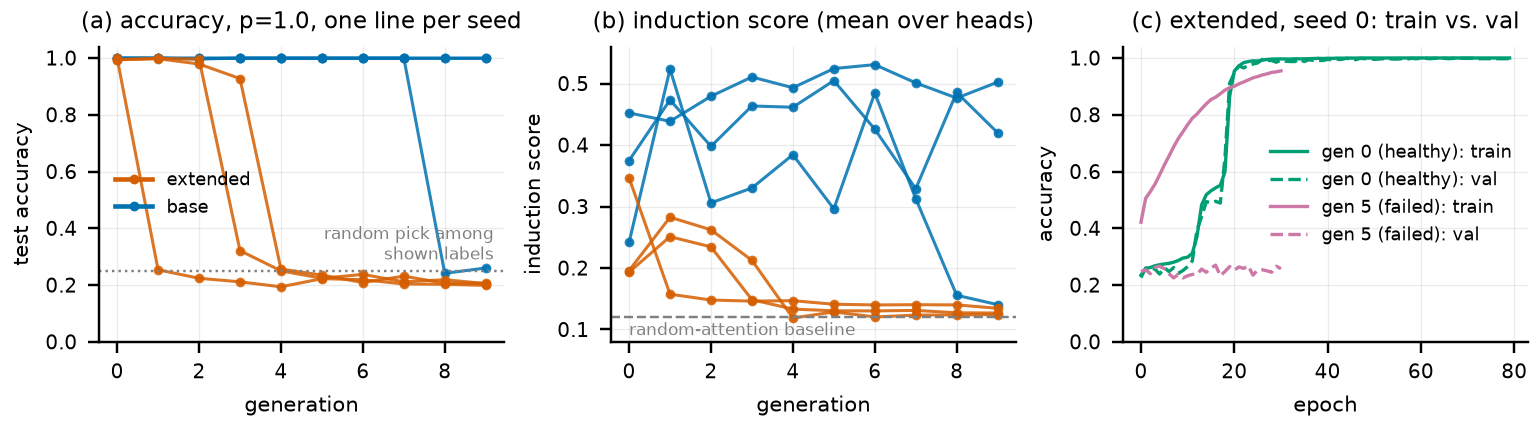
\includegraphics[width=\textwidth]{figures/fig_main.png}
  \caption{Extended-variant collapse is abrupt and absorbing, with a
  memorisation signature. (a,\,b) One line per seed at $p{=}1$; dotted line:
  guessing among the 4 labels shown in context. (c) Seed 0: a failed
  generation fits its training pool (solid) but not validation data
  (dashed); a healthy one does both.}
  \label{fig:main}
\end{figure*}

\begin{figure*}[t]
  \centering
  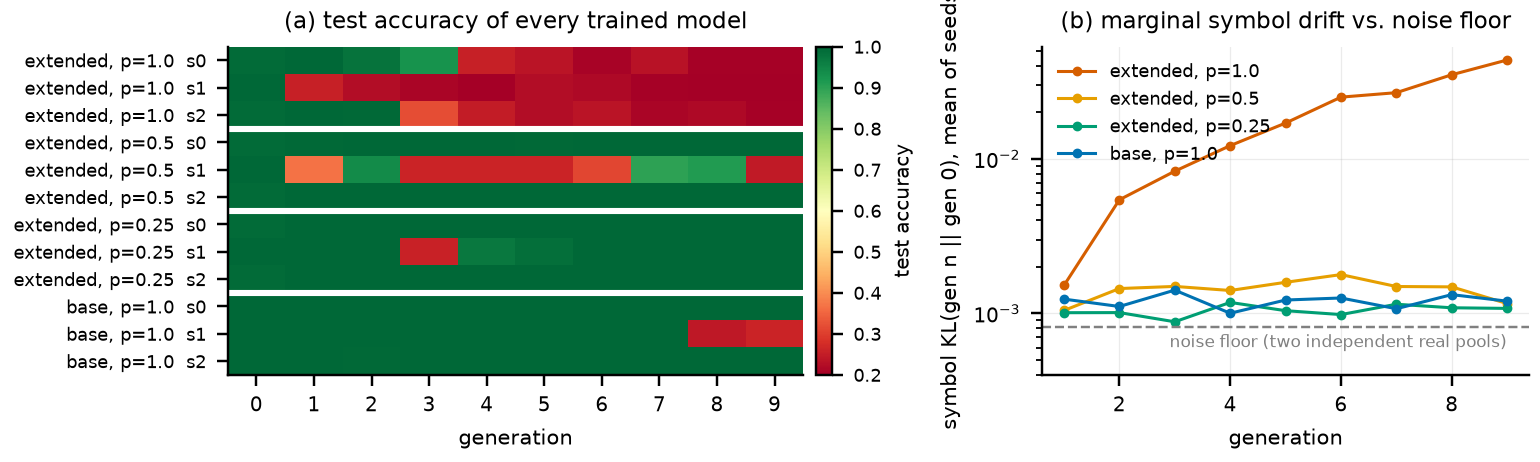
\includegraphics[width=\textwidth]{figures/fig_failure_map.png}
  \caption{(a) Test accuracy of all 120 collapse-run models: failures occur
  in every seed at $p{=}1$ but in a single seed for $p{<}1$ and the base
  variant. (b) Mean symbol KL to generation 0 (log scale): only $p{=}1$
  rises clearly above the noise floor, and it is still small when accuracy
  has already collapsed.}
  \label{fig:map}
\end{figure*}

\section{Results}
\looseness=-1
\textbf{Sanity check.} All six no-collapse runs reach $\geq$99.4\% test
accuracy (base: 100\%) after an abrupt jump in validation accuracy at epoch
10--28, the induction phase change (Supp.\ Table~\ref{tab:sanity}).
\textbf{Collapse is abrupt and absorbing} (Figs.~\ref{fig:main}a,
\ref{fig:map}a). At $p{=}1$ the extended model falls from 99.5\% (generation
0) to $\approx$20\% in all three seeds, first failing at generation 4, 1
and 3, and no seed recovers (22 of 27 models fail, i.e.\ test accuracy
$<$0.5; Supp.\ Table~\ref{tab:fail}). Test loss rises from 0.015 to 5.7 nats (uniform guessing: 2.08):
failed models are confidently wrong. Only one seed shows a graded precursor
(0.998$\to$0.979$\to$0.928$\to$0.256). \textbf{The circuit disappears}
(Fig.~\ref{fig:main}b): the induction score falls from 0.245 to 0.128
(baseline 0.120), the previous-token score from 0.185 to 0.139, and
attention entropy rises from 1.33 to 2.00 nats (maps: Supp.\ Fig.~\ref{fig:attn}).
\textbf{Memorisation replaces induction} (Fig.~\ref{fig:main}c): across the
22 failed models, training accuracy reaches 0.96 on average while validation
accuracy peaks at 0.27 on average (never above 0.32) and validation loss rises
steadily after the first epochs; healthy models reach 1.00 and 0.99--1.00. \textbf{Real data helps, and the base
variant is not immune} (Fig.~\ref{fig:map}a). At $p{=}0.25$ 1 of 27 models
fails; at $p{=}0.5$, 6 of 27, with recoveries. All 9 failures at $p{<}1$ or
in the base variant occur in seed 1. The base variant, expected to show weak
collapse, is healthy in 25 of 27 models, but when it fails (seed 1,
generations 8--9) the failure is as complete as the extended model's.
\textbf{Marginal drift is a weak predictor} (Fig.~\ref{fig:map}b). At $p{=}1$
symbol KL grows from 0.0015 to 0.044 nats (54$\times$ the floor) and symbol
entropy falls by only 1\% (4.158$\to$4.115, maximum 4.159), yet the pools
that first triggered failure had KL of just 0.0025--0.0034 (3.1--4.2$\times$ the
floor), and failed generations at $p{<}1$ sit at 1.0--3.6$\times$ the floor.

\section{Discussion}
\looseness=-1
\textbf{Collapse here behaves like a bifurcation, not erosion.} Outcomes are
bimodal: a trained model either has the circuit (accuracy $\approx$1) or
lacks it ($\approx$0.2). That contrasts with the gradual tail loss
characterising collapse in generative models \citep{shumailov2024ai}, and is
consistent with induction heads forming through an abrupt phase change
\citep{olsson2022incontext,singh2024needs}. We hypothesise that perturbed
training data pushes optimisation into a regime where fitting the pool is
easier than learning the general rule, after which the model never
generalises; at $p{=}1$ failure is absorbing, plausibly because a failed
generator's samples are poor training data. \textbf{Answering the question.}
The circuit degrades (scores at baseline, diffuse attention), and what
replaces it is memorisation of the training pool, not of the task mapping,
which relabelling makes impossible. \textbf{Marginal statistics are nearly
blind.} Entropy and KL, our analogue of tail loss, barely moved while ICL
vanished, so a model could look healthy in distribution yet have lost the
circuit. The damage must lie in sample \emph{structure} that marginals
cannot see, such as inconsistent labels for a repeated symbol or wrong repeat
counts; the extended model's next-symbol head is 14\% below the Bayes-optimal
accuracy (0.326 vs.\ 0.380), consistent with imperfect repeat structure. We
did not test this, as dataset snapshots were not retrieved.
\textbf{Limitations.} (i) Three seeds, and every failure at $p{<}1$ is in
one initialisation, so failure probabilities are not estimable; the real-data
pool is shared across seeds. (ii) Generations $\geq$1 use size-matched
resamples with replacement ($\approx$63\% distinct sequences) and healthy
later generations reach 90\% validation accuracy sooner than generation 0
(medians 4--9 vs.\ 19 epochs in extended runs, 7 vs.\ 11 in base; Supp.\
Table~\ref{tab:t90}); without a $p{=}0$ control we cannot say how much this
matters, although the mostly healthy base and $p{=}0.25$ runs share it. (iii) Failed runs were early-stopped after 31--43 epochs, so a delayed
transition is not excluded. (iv) Scores average all heads; our per-head
ablation and influence-proxy tools were not applied to the collapse
checkpoints. (v) A symbolic task, a tiny model, and final-epoch weights
(which inflate loss).

\section{Acknowledgements (Not in Page Limit)}
Computations were performed using High Performance Computing infrastructure
provided by the Mathematical Sciences Support Unit at the University of the
Witwatersrand.

\section{Contribution Statements (Not in Page Limit)}
% TODO(author): to be written by the authors; all group members must agree.
[To be completed by the author(s).]

\bibliographystyle{apacite}
\setlength{\bibleftmargin}{.125in}
\setlength{\bibindent}{-\bibleftmargin}
\bibliography{references}

\newpage
% ============================================================================
% PLACEHOLDER -- NOT THE REAL NEURIPS 2024 CHECKLIST
% ============================================================================
% The project brief requires the official NeurIPS 2024 ethics
% statement/questionnaire, to be posted on Moodle by the course instructor,
% appended here verbatim. That file was not available at the time this
% repository was assembled, so its content has NOT been fabricated -- this
% is a structural placeholder only.
%
% TODO (author, before submission):
%   1. Download the official NeurIPS 2024 checklist .tex from Moodle.
%   2. Replace this entire file's contents with it.
%   3. Draft answers for the standard checklist topics, written from what the
%      project actually did, are in ethics/neurips_checklist_draft_answers.md;
%      copy them over after checking each question's wording.
%   4. Fill in each checklist item honestly based on the actual project
%      (task/data are synthetic and symbolic, no human subjects, no
%      personally identifiable data, small-scale reproducibility-focused
%      compute -- but answer from the real checklist's actual wording, not
%      this summary).
% ============================================================================

\section*{NeurIPS 2024 Ethics / Reproducibility Checklist (PLACEHOLDER)}
\textit{This section must be replaced with the official checklist from
Moodle before submission. Do not submit this placeholder as-is.}


\newpage
\section*{Faculty of Science AI Ethics Statement}
% Kept in sync by hand with ../ethics/ai_ethics_statement.md.
Generative AI (Claude, Anthropic) was used to assist with this project
under the supervision and direction of the human author(s), who take full
responsibility for the final content.

\textbf{Code.} Claude was used as a pair-programming assistant to help
design and implement the codebase in \texttt{src/} (the synthetic
in-context-learning task generator, the transformer model, the training
loop, the model-collapse generation pipeline, and the interpretability
tooling), following an architecture and experimental design specified by
the author(s) from the project brief and the cited literature. All code
was written from first principles for this project; no code was copied
from the reference implementation (\texttt{aadityasingh/icl-dynamics}) or
any other external repository. The author(s) reviewed, ran, and verified
the code and its outputs, including an induction-head phase-transition
sanity check, before proceeding to the full experiment suite.

\textbf{Writing and analysis.} Claude was used to help analyse the
experimental logs and to draft and edit this extended abstract. All reported
numbers and figures are computed by \texttt{experiments/analyze\_results.py}
from the logs produced by the code in this repository -- none were
fabricated or estimated by the AI assistant. The author(s) reviewed and take
responsibility for all claims, interpretations, and conclusions in this
document.

\textbf{Verification.} No results, citations, or technical claims in this
abstract were accepted without the author(s) independently checking them
against the actual experimental logs and figures.

\textit{(Author(s): please review and edit this statement to accurately
reflect your own usage before submission, per course policy.)}

%==========================================================================
\clearpage
\setcounter{figure}{0}\setcounter{table}{0}
\renewcommand{\thefigure}{S\arabic{figure}}
\renewcommand{\thetable}{S\arabic{table}}
\section*{Supplementary Material}

\subsection*{S1. Setup, provenance and reproducibility}
\textbf{Configuration.} $K{=}64$, $L{=}8$, 4 exemplars $\times$ 3 repeats
(12 context pairs, sequence length 25); 2 layers $\times$ 4 heads,
$d_\text{model}{=}64$, $d_\text{ff}{=}256$; AdamW, learning rate $10^{-3}$,
weight decay 0.1, batch 128, 100 warm-up steps with cosine decay, gradient
clipping 1.0; at most 100 (base) or 80 (extended) epochs with early stopping
on validation loss (patience 40 and 30 respectively); 20{,}000 training
sequences per generation, 800 validation and 800 test sequences from the true
distribution. Seeds 0, 1, 2 set initialisation and sampling randomness; the
real-data pool seed is shared across seeds. Training ran on mscluster as
Slurm array jobs; no GPU was requested, and the code selects the device
automatically.

\textbf{Provenance.} All 18 (experiment, seed) runs finished. In the first
submission of the medium group (job 62527), 6 of 9 tasks crashed at start-up
with a \texttt{FileExistsError}: parallel tasks raced to create the shared
directory \texttt{results/collapse/}. They wrote no results and were
resubmitted unchanged as job 62798 (the race is now fixed with
\texttt{os.makedirs}). The other groups ran as jobs 62521 (fast) and 62535
(slow). Generation 0 of every collapse run reproduces the matching no-collapse
run (test accuracy identical in 6 of 6 pairs; induction score identical in 5
of 6, the sixth differing by 0.0006 because that no-collapse log's last
snapshot predates early stopping), confirming determinism across jobs. Exact commands are in \texttt{README.txt}; every number in this
document is computed by \texttt{experiments/analyze\_results.py}.

\textbf{Pilot observation (not part of the reported results).} With
4{,}000-sequence pools, some initialisations (and a pool with 0.4\% label
noise) memorised the training set instead of learning induction even without
collapse; with 20{,}000 sequences a previously failing seed reached 100\%
accuracy and 1\% injected label noise still gave 99.6\%. Those pilot logs
were not retained, so we report this as motivation for the pool size only.

\begin{table*}[h]
\centering\footnotesize
\caption{No-collapse sanity runs. ``Epoch to 0.9'': first epoch with
validation accuracy $>$0.9. Induction score is averaged over all 8 heads
(random baseline 0.12). The last row is the Bayes-optimal accuracy of the
auxiliary heads under the true generating process, computed by simulation.}
\label{tab:sanity}
\begin{tabular}{@{}llccccc@{}}
\toprule
Model & Seed & Test acc. & Epoch to 0.9 & Induction score & Next-label acc. & Next-symbol acc.\\
\midrule
base     & 0 & 1.000 & 10 & 0.452 & -- & --\\
base     & 1 & 1.000 & 23 & 0.241 & -- & --\\
base     & 2 & 1.000 & 11 & 0.375 & -- & --\\
extended & 0 & 0.994 & 19 & 0.196 & 0.713 & 0.306\\
extended & 1 & 0.999 & 12 & 0.347 & 0.719 & 0.315\\
extended & 2 & 0.994 & 28 & 0.193 & 0.710 & 0.358\\
\midrule
Bayes-optimal & -- & -- & -- & -- & 0.720 & 0.380\\
\bottomrule
\end{tabular}
\end{table*}

\subsection*{S2. Failure counts and training dynamics}
\begin{table*}[h]
\centering\footnotesize
\caption{Per condition: models with test accuracy $<$0.5 among the 27
trained at generations 1--9 (3 seeds), the first failing generation per seed,
and mean training dynamics of failed vs.\ healthy models (final train
accuracy / maximum validation accuracy over epochs / epochs run).}
\label{tab:fail}
\begin{tabular}{@{}lcccll@{}}
\toprule
Condition & Failed & Seeds hit & First failing gen.\ (s0/s1/s2) & Failed: train / max val / epochs & Healthy: train / max val / epochs\\
\midrule
extended, $p{=}1.0$  & 22/27 & 3 & 4 / 1 / 3 & 0.957 / 0.268 / 31.5 & 1.000 / 0.992 / 74.0\\
extended, $p{=}0.5$  &  6/27 & 1 & -- / 1 / -- & 0.813 / 0.290 / 35.3 & 1.000 / 0.989 / 72.7\\
extended, $p{=}0.25$ &  1/27 & 1 & -- / 3 / -- & 0.811 / 0.273 / 37.0 & 1.000 / 0.999 / 75.6\\
base, $p{=}1.0$      &  2/27 & 1 & -- / 8 / -- & 0.895 / 0.280 / 42.5 & 1.000 / 1.000 / 98.0\\
\bottomrule
\end{tabular}
\end{table*}

\subsection*{S3. An unexplained effect: later generations learn faster}
\begin{table}[h]
\centering\footnotesize
\caption{Median epoch at which validation accuracy first exceeds 0.9, for
generation 0 and for healthy models of generations $\geq$1 (same seeds, same
initialisation).}
\label{tab:t90}
\begin{tabular}{@{}lcc@{}}
\toprule
Condition & Gen.\ 0 & Healthy gen.\ $\geq$1\\
\midrule
extended, $p{=}1.0$  & 19 & 9\\
extended, $p{=}0.5$  & 19 & 4\\
extended, $p{=}0.25$ & 19 & 4\\
base, $p{=}1.0$      & 11 & 7\\
\bottomrule
\end{tabular}
\end{table}
Healthy later generations reach the induction transition roughly
1.6--4.8$\times$ sooner than generation 0, even in the base variant, whose
contexts are real and whose labels differ from the true ones only through the
model's rare mistakes. The only structural difference
we know of is that generations $\geq$1 are built by sampling with
replacement from a size-matched pool ($\approx$63\% distinct sequences),
whereas generation 0 uses 20{,}000 distinct sequences. We did not isolate the
cause. A $p{=}0$ control (real data resampled the same way) and a
without-replacement variant would settle whether resampling, rather than
synthetic content, drives it; neither was run.

\subsection*{S4. Qualitative figures}
\begin{figure*}[h]
  \centering
  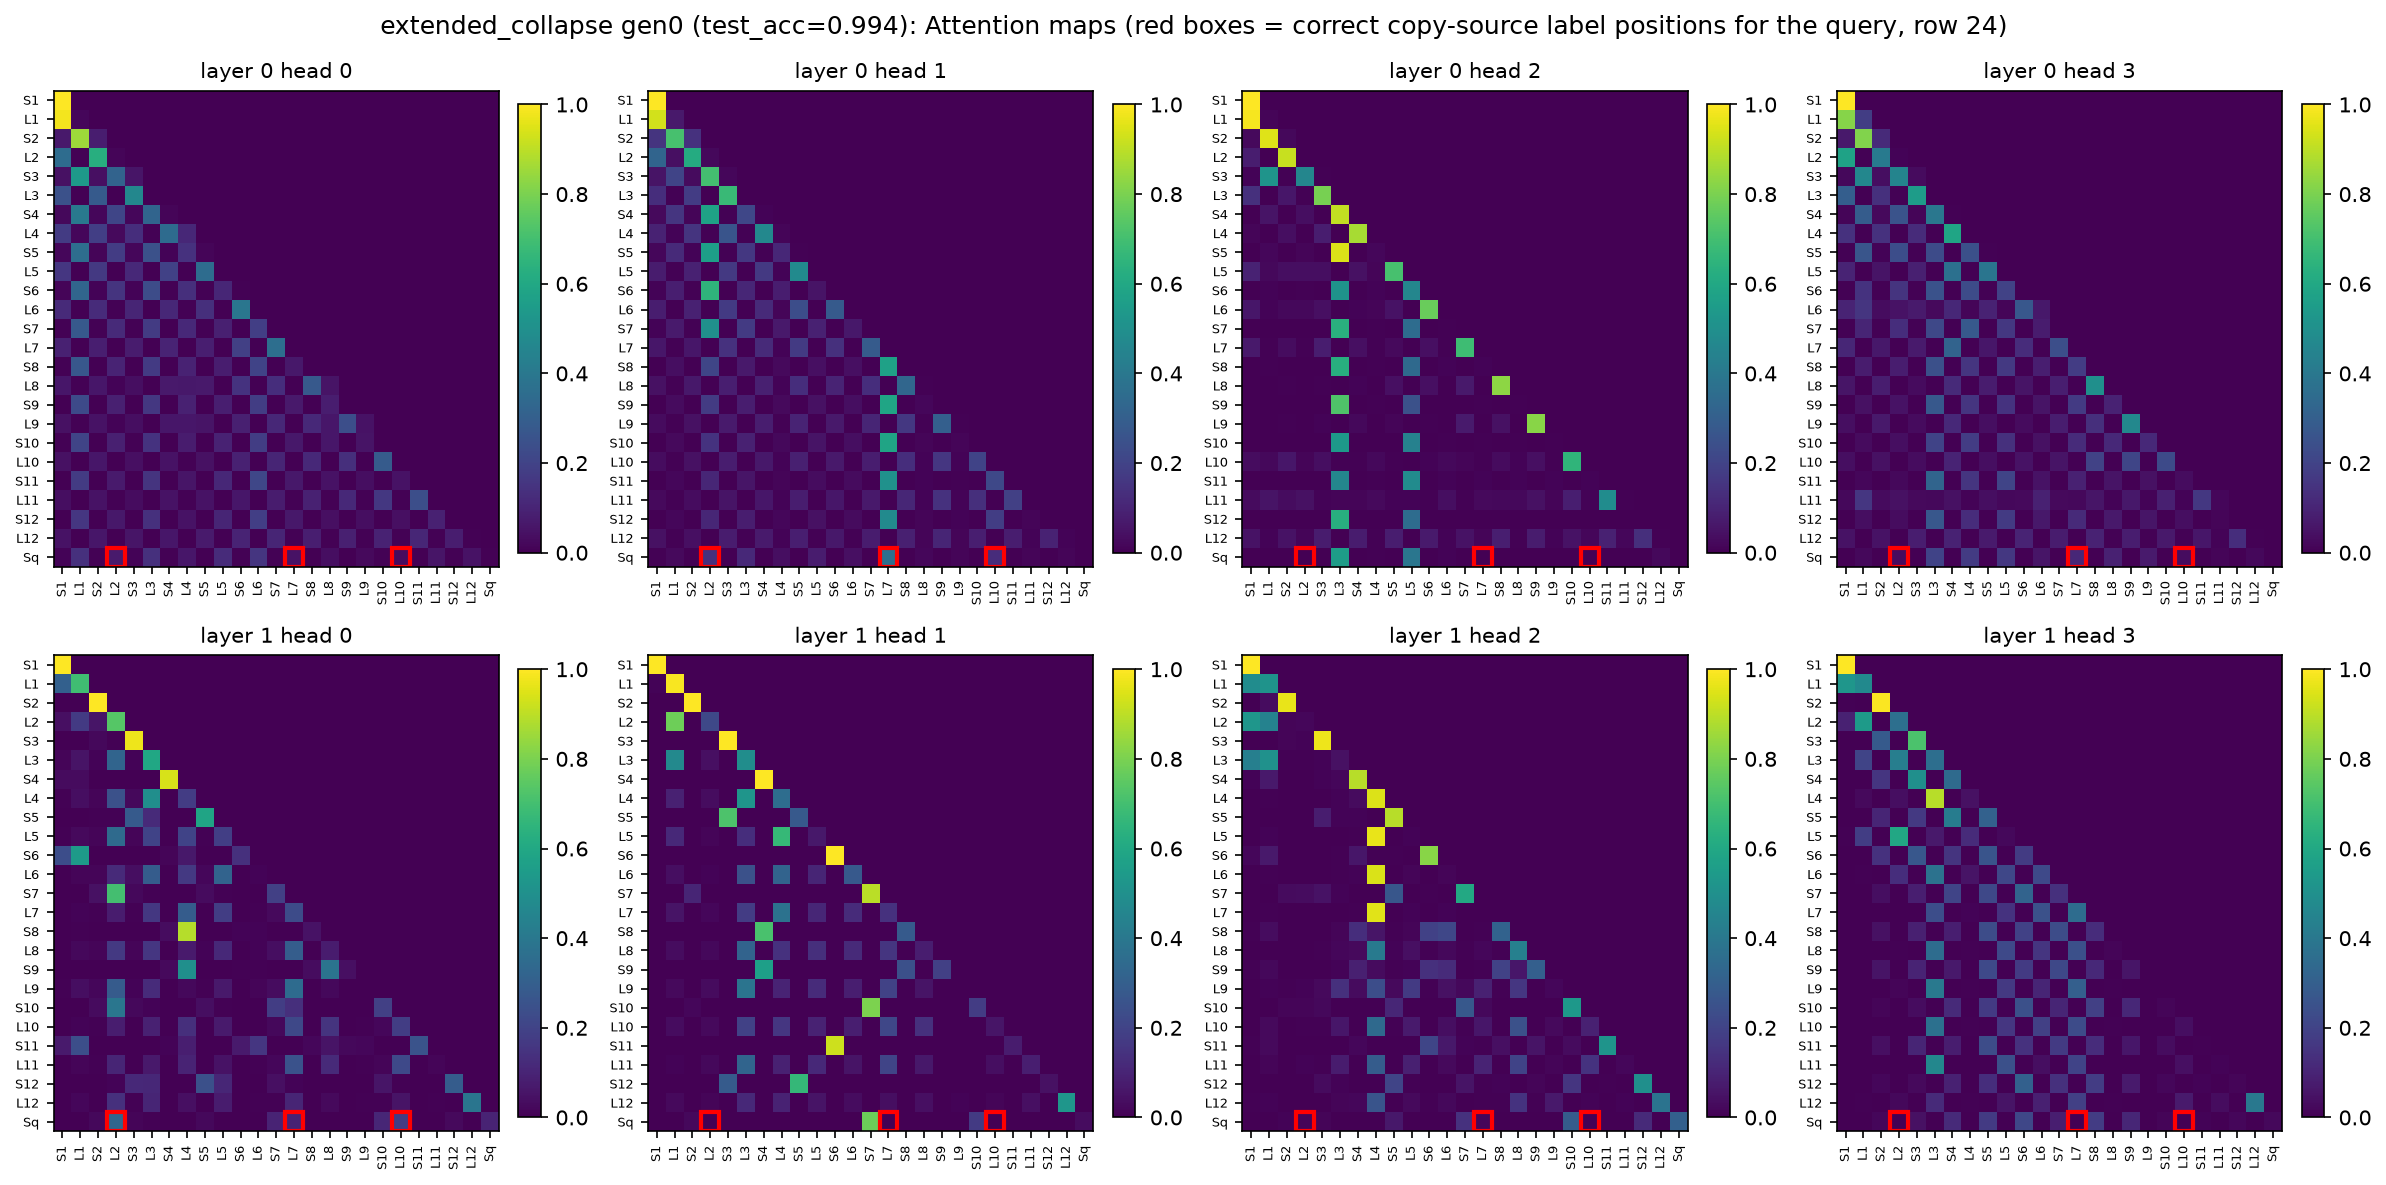
\includegraphics[width=0.92\textwidth]{figures/attn_extended_collapse_gen0.png}\\[2pt]
  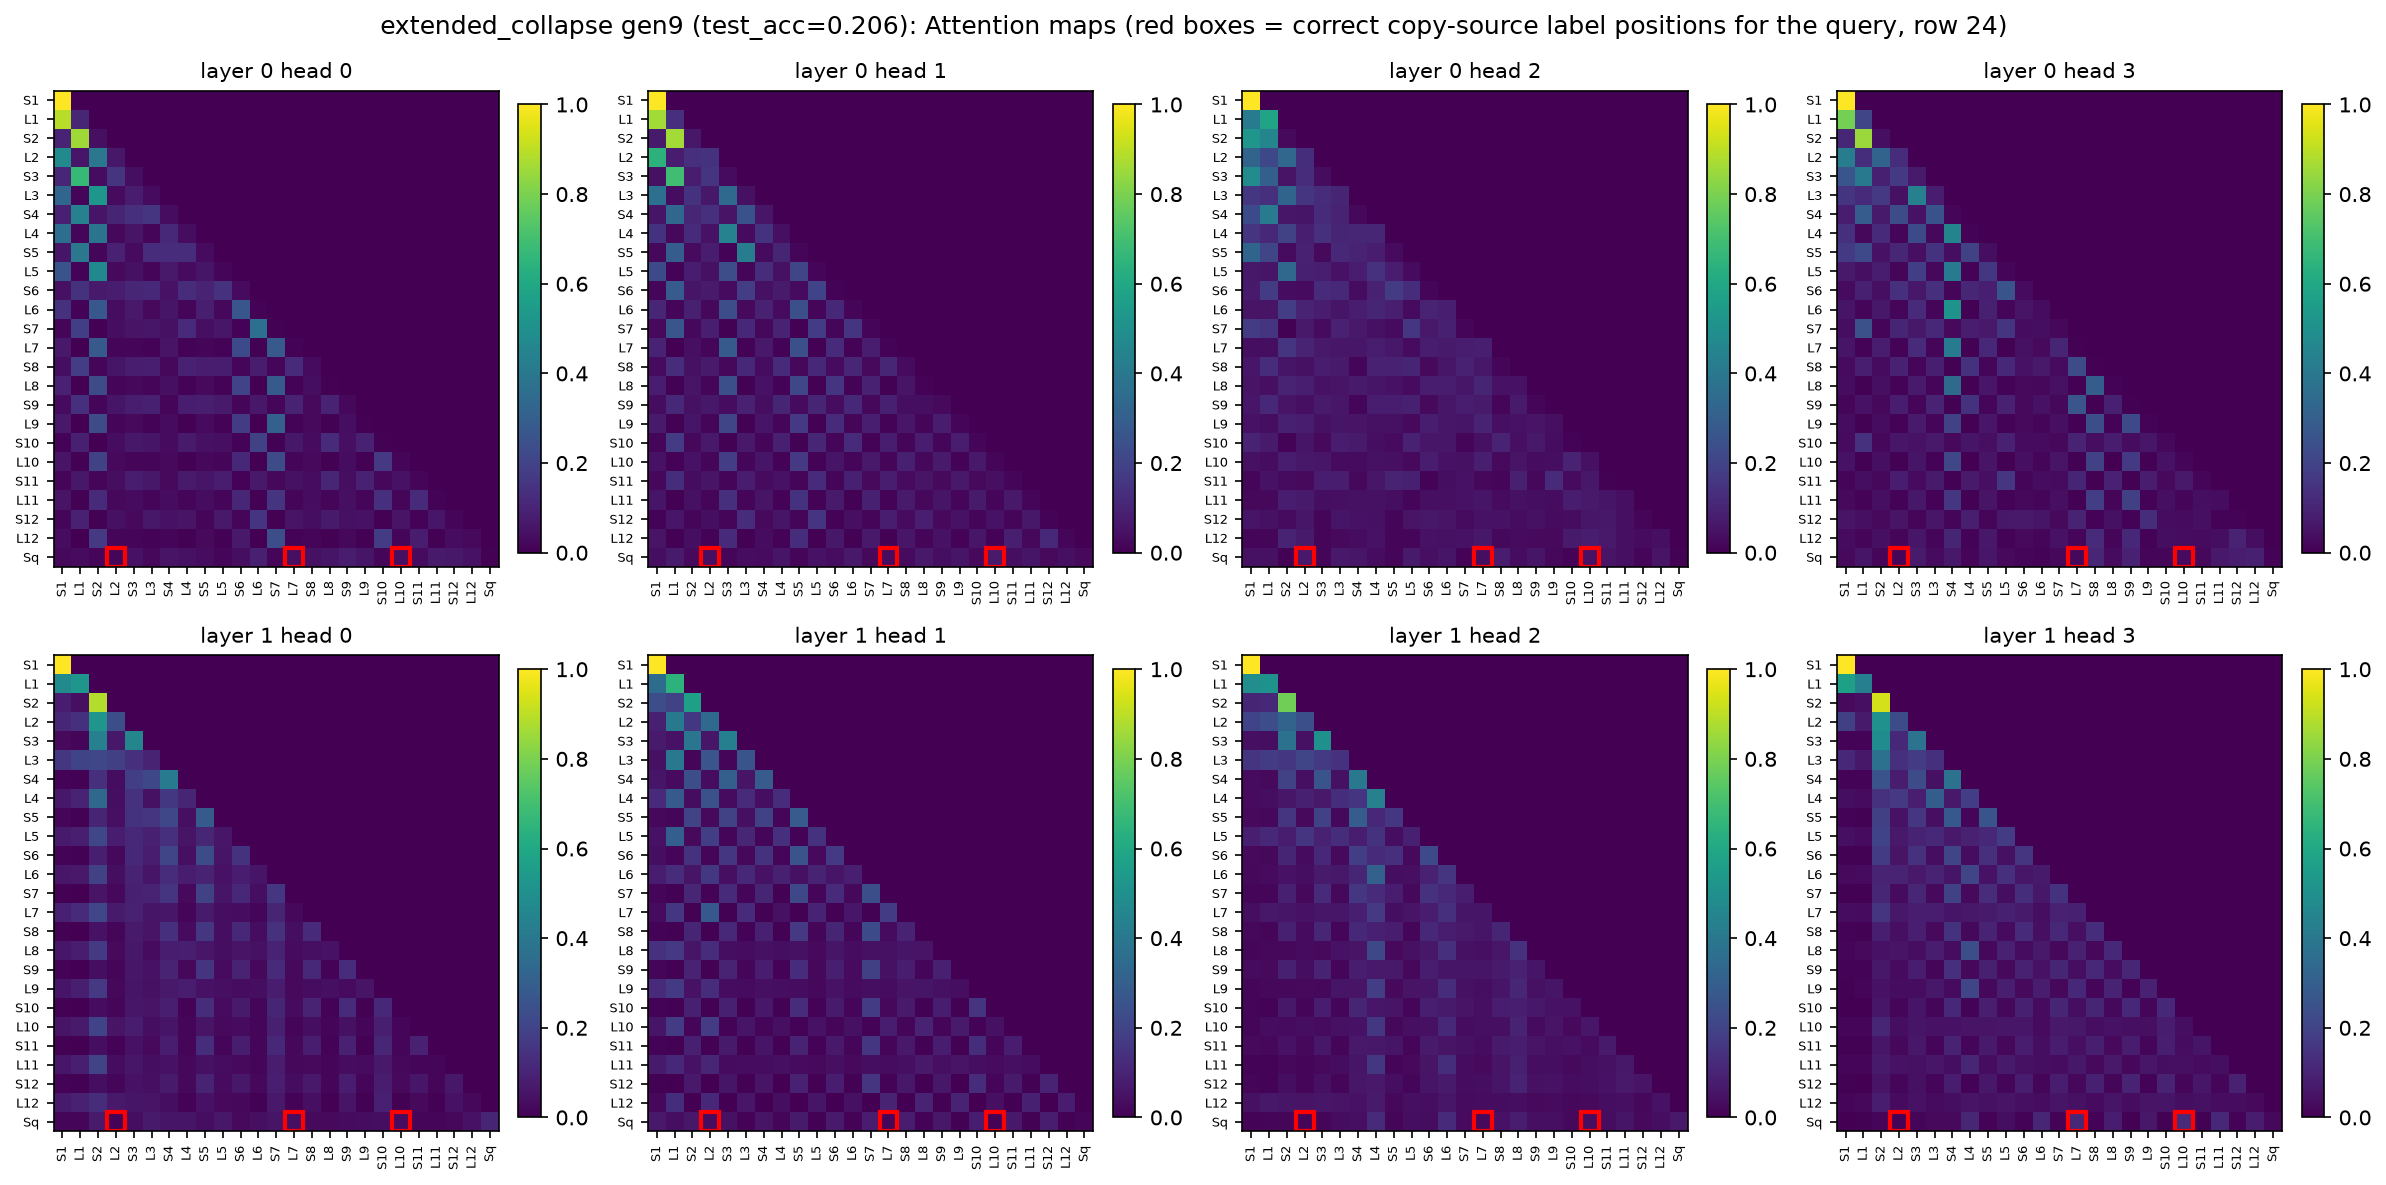
\includegraphics[width=0.92\textwidth]{figures/attn_extended_collapse_gen9.png}
  \caption{Attention maps for one example (seed 0, extended, $p{=}1$) at
  generation 0 (top, test accuracy 0.994) and generation 9 (bottom, 0.206);
  red boxes mark the correct copy-source label positions for the query (last
  row). At generation 0 attention is sharply structured, though in most
  heads the query row puts only modest mass on the red boxes, so we do not
  claim a single clean induction head from one example; by generation 9
  every head is diffuse. Generated on the cluster from checkpoints that were
  not retrieved, so these figures cannot be regenerated locally.}
  \label{fig:attn}
\end{figure*}

\begin{figure}[h]
  \centering
  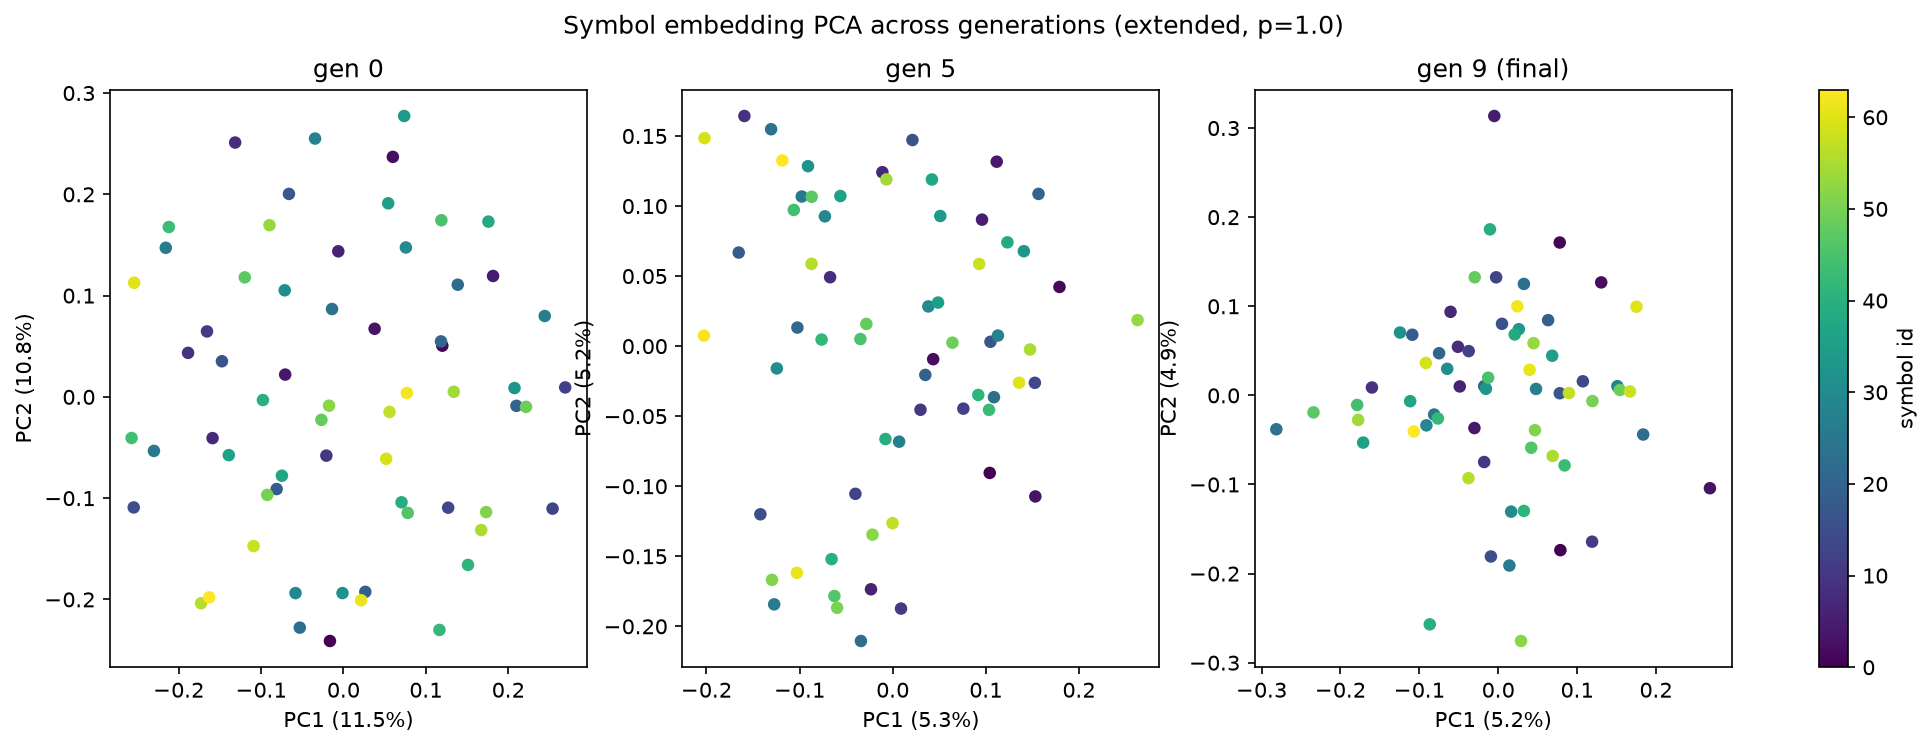
\includegraphics[width=\columnwidth]{figures/embedding_pca_extended_collapse.png}
  \caption{PCA of the symbol-embedding table at generations 0, 5 and 9 (seed 0,
  extended, $p{=}1$). No structure is visible at any generation (symbols are
  interchangeable by design); the leading component explains less variance
  later (11.5\% $\to$ 5.2\%), which we do not interpret. A negative,
  uninformative result.}
  \label{fig:pca}
\end{figure}

\subsection*{S5. Not done, and what would strengthen the work}
None of the following is reflected in the results above. Tooling for each now
exists in the repository (see \texttt{README.txt}, Section 6g) but had not been
run when this was written; if it has been, the numbers and Limitations above
must be updated to match. (1) Per-head ablation (a simplified ACDC-style
sweep, \texttt{src/circuits.py}) and best-single-head induction scores per
generation (\texttt{experiments/analyze\_circuits.py}); the gradient-influence
proxy (\texttt{src/attribution.py}, inspired by Chen et al.) has not been
applied to the collapse runs. (2) A structure-aware drift measure (label
consistency for repeated symbols, repeat counts, label injectivity) on each
generation's training pool, which would test the structural-corruption
hypothesis directly (\texttt{analyze\_circuits.py}; recorded automatically in
new runs). (3) Retraining the first failed generation of each failing run with
early stopping disabled, to settle whether any failure is a delayed transition
(\texttt{experiments/retrain\_generation.py}). (4) Controls for the duplicate-
sequence resampling confound ($p{=}0$ with and without resampling, and the
$p{=}1$ experiment without duplicates), and five more seeds with independent
real-data pools.
\end{document}
